%
% software.tex
%
% Copyright (C) 2015, Achim Lösch <achim.loesch@upb.de>, Christoph Knorr <cknorr@mail.uni-paderborn.de>
% All rights reserved.
%
% This documentation may be modified and distributed under the terms
% of the BSD license. See the LICENSE file for details.
%
% encoding: UTF-8
% tab size: 4
%
% author: Achim Lösch (achim.loesch@upb.de)
% created: 7/24/14
% version: 0.5.8 - change project name to ampehre
%          0.6.0 - add ioctl for the ipmi timeout, new parameters to skip certain measurements 
%                  and to select between the full or light library. 
%

\section{Protocol}\label{sec:Protocol}

In order to enable communication between client and server, a protocol had to be defined. Our protocol is based on \texttt{http}. Connections are established via TCP/IPv4 network protocol.

\subsection{Message Types}
An important part of a message is the type, so that server and client know how to deal with the incoming information. The following message types are currently implemented:
 

\begin{center}
	\begin{tabularx}{.9\textwidth}{|>{\hsize=.16\textwidth}X|X|}
		\hline
		\textbf{Option} & \textbf{Description} \\ \hline
		\texttt{CLIENT\_REG} & The first contact is initiated by the client. This is an attempt to register a client to the server. Skipping this step leads to the server refusing to answer.\\ \hline
		\texttt{SET\_FREQ} & The client receives the sampling frequencies for each computing resource from the heterogeneous node.\\ \hline
		\texttt{DATA\_REQ} & After the registration, the client can request measured data from the server.\\ \hline
		\texttt{DATA\_RES} & The server responds to a specific data request.\\ \hline
		\texttt{TERM\_COM} & The communication is terminated from either side.\\ \hline
	\end{tabularx}
\end{center}

\subsection{Communication}

The flow diagram (Figure \ref{fig:protocol}) shows a typical sequence of events, forming a communication between server and client.
\begin{center}
	\begin{figure}
		\begin{center}
			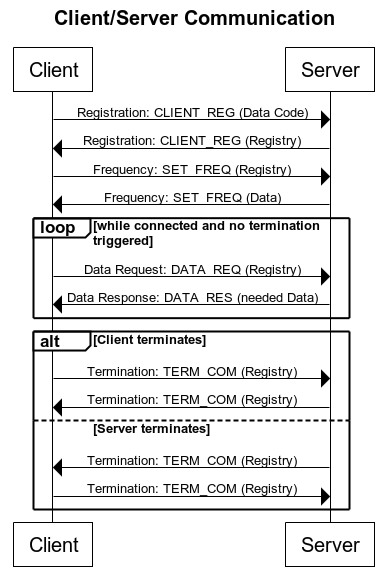
\includegraphics[width=0.8\textwidth]{protocol.png} 
			\caption{Protocol flow diagram}
			\label{fig:protocol}
		\end{center}
	\end{figure}
\end{center}
First of all the client registers to the server, transmitting a value of datatype long. This value contains the information about which data is needed and which is not. The server answers with a unique registry value.\newline
Afterwards the sampling frequencies of the hardware are transmitted to the client.\newline
Then the data needed for the graphs is being requested by the client as long as necessary.\newline
The connection is finally terminated by either the client or the server.\newline


\subsection{Message Structure}
A message consists of a header, which contains the message type and protocol version. The second part is the body, which contains the message. A tail is not defined.

\subsubsection{Header}

The following shows the header for a client registration:
\begin{lstlisting}[caption={A MSMonitor Protocol Header}, label=lst:HeaderMSMP]
CLIENT_REG / MSMP/0.1
\end{lstlisting}
It consists of the message type, followed by the protocol name and version. In general message types give the client and server information about how to interpret the message body of the current message.\newline
Please notice the resemblance to the widely known HTTP header:
\begin{lstlisting}[caption={A HTTP Header}, label=lst:HeaderHTTP]
GET /file.html HTTP/1.1
\end{lstlisting} 


\subsubsection{Body}

The message body generally highly depends on its type. This is the message body of the CLIENT\_REG message.
\begin{lstlisting}[caption={Client registers to server}, label=lst:msg]
CLIENT_REG / MSMP/0.1
0b1101000000000000010000000000000000000000000000000000000000000000
\end{lstlisting}
The value of datatype long, indicates which data is being requested. Each Bit set to '1' means, that the corresponding value is needed and '0', that it is not. The server will only send back those values, which are requested by the client. In this case it would be only four values. Please note, that it is a long value which is being transmitted. It is presented human readable in order to clarify the principle.\newline
Please refer to \textit{Protocol.c} in order to understand the bitfield.\newline
\begin{lstlisting}[caption={Server registers client}, label=lst:msg1]
CLIENT_REG / MSMP/0.1
REG: 0
\end{lstlisting}
The server accepts the client and registers it with the unique id '0'. Now the client can request data by transferring its unique registration ID.\newline
\begin{lstlisting}[caption={Client requests data}, label=lst:msg2]
DATA_REQ / MSMP/0.1
REG: 0
\end{lstlisting}
As the client is registered to the server, the server sends data to the client according to the data request bitfield mentioned in Listing \ref{lst:msg}.\newline
\begin{lstlisting}[caption={Server responds with needed data}, label=lst:msg3]
DATA_RES / MSMP/0.1
201.58
365
17
23
\end{lstlisting}
The server responds with the requested data in a defined order, which is equally known by server and client. The data is of datatype double. Please note, the message is usually not human readable.\newline
The DATA\_REQ and DATA\_RES messages are sent/received in a loop until one of the subscribers terminates the communication by sending a TERM\_COM message and disconnects.
\begin{lstlisting}[caption={Client terminates communication}, label=lst:msg4]
TERM_COM / MSMP/0.1
REG: 0
\end{lstlisting}

